\documentclass[a4paper]{article}
\usepackage{enumerate}
\usepackage{amsmath}
\usepackage[english]{babel}
\usepackage{url}
\usepackage{graphicx}

\title{Naive Bayes\\\large Lab Session 1\\Machine Learning: Pattern Recognition\\Master Artificial Intelligence}

\author{Camiel Verschoor \\StudentID: 10017321\\UvAnetID: 6229298\\ \url{Verschoor@uva.nl} \and Steven Laan\\StudentID: 6036031\\UvAnetID: 6036031\\\url{S.Laan@uva.nl}}

\begin{document}

\maketitle

\section{Feature Selection}

\subsection{Smoothing}
\subsubsection{Add-$\lambda$ smoothing}

\subsubsection{Good-Turing discounting (?)}


\subsection{Selection criterion}
\subsubsection{Linear}
$$f(x,y) = |x-y|$$

\subsubsection{Zipf}
When dealing with natural language, the law of Zipf has to be taken into account. This law or probability distribution shows that there are only a couple of words that have a high frequency. Moreover, the most frequent word has a frequency nearly twice as high as the second most frequent. On the other hand, there is massive amount of words that have only been observed once. The zipf distribution then tells us that there is an even bigger amount of words that haven't even been observed once. 
When plotted on a double logirithmic scale, also known as loglog-scale, the Zipf distribution is a straight line. In figure \ref{fig:ZipfDistribution} it can be seen that the data used for training follows a Zipf distribution, as it is more or less a straight line when plotted on a double logarithmic scale.

\begin{figure}
\centering
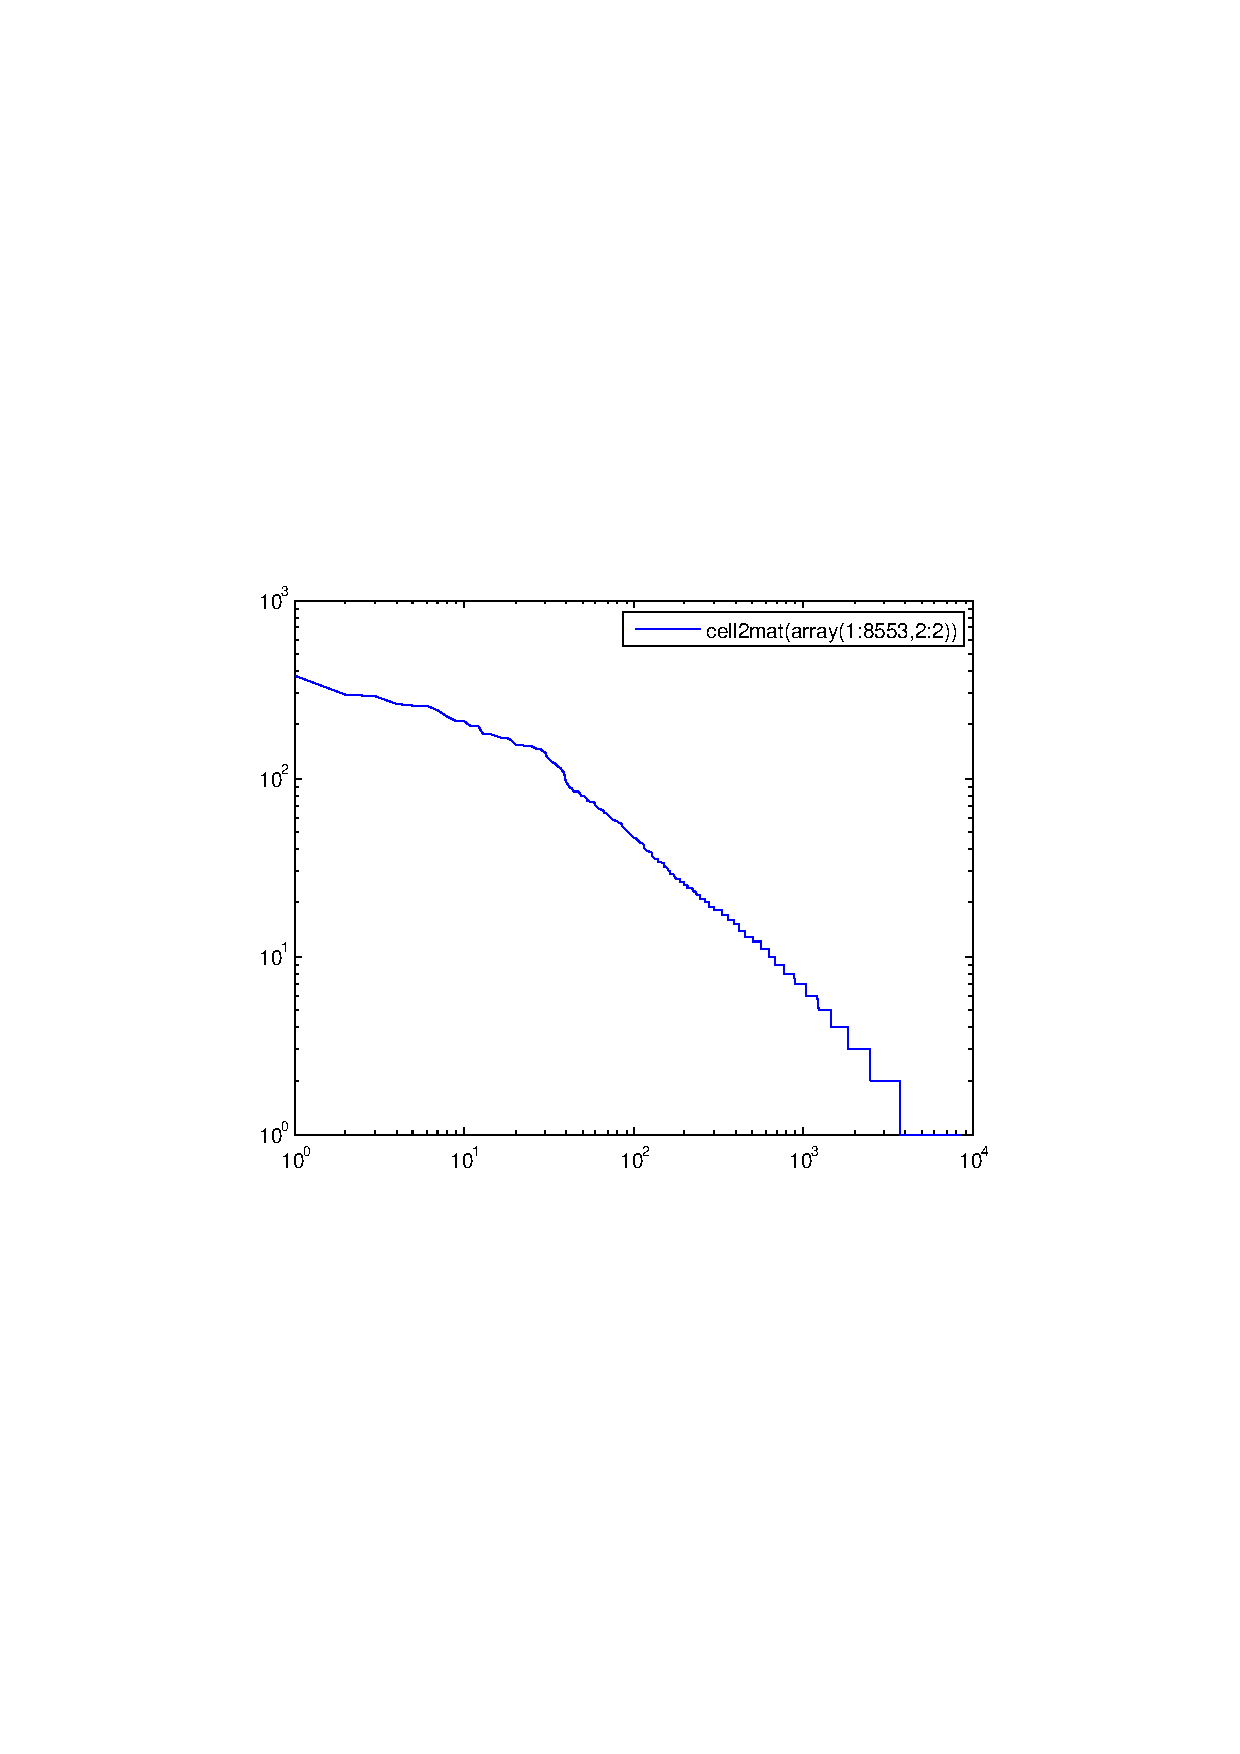
\includegraphics{zipfLaw.pdf}
\caption{The frequencies of the words in the trainingset plotted on double logarithmic scale.}
\label{fig:ZipfDistribution}
\end{figure}

Based on this distribution, it is probably a better idea to do something with this distribution, instead of discounting in linear fashion.

Therefore, we created the following function:
$$f(x,y) = \frac{1}{1-|x-y|}$$

\end{document}